
\section{Το πρόγραμμα LASOR (2005), ΗΠΑ}

Στην αρχιτεκτονική LASOR, οπτικά πακέτα των 40 Gbps δρομολογούνται με
βάση το μήκος κύματος του πακέτου και τις οπτικές ετικέτες των 10
Gbps. Η ενσωμάτωση της λειτουργίας μεταγωγής και δρομολόγησης σε PIC
επιτρέπει την πραγματοποίηση βελτιωμένων λειτουργιών δρομολόγησης στο
οπτικό πεδίο, ενώ προσφέρει πλεονεκτήματα της ολοκλήρωσης
συμπεριλαμβανομένων των μειωμένων απαιτήσεων ισχύος και μεγέθους.

Τα βασικά συστατικά του οπτικού δρομολογητή LASΟR \cite{1584172} είναι
μια δομή εναλλαγής πακέτων (packet switching fabric), ένας οπτικός
ενταμιευτής, ένα στοιχείο δρομολόγησης ανίχνευσης μήκους κύματος
(wavelength sensitive routing element) και ένα στοιχείο αναγέννησης
δεδομένων.

Ο εναλλάκτης πακέτων μετατρέπει τα οπτικά πακέτα σε άλλο μήκος
κύματος, βάση των πληροφοριών που βρίσκονται σε έναν lookup table. Ο
οπτικός ενταμιευτής χρησιμοποιείται για τη διευθέτηση των συγκρούσεων
μεταξύ πακέτων που οδεύουν στην ίδια θύρα εξόδου. Ένα στοιχείο
δρομολόγησης ανίχνευσης μήκους κύματος συνδυάζεται με έναν all-optical
μετατροπέα μήκους κύματος, με σκοπό την προώθηση πακέτων απ τους
ενταμιευτή των εισόδων στις θύρες εξόδου. Αυτά τα στοιχεία
συμπεριλαμβάνουν integrated tunable wavelength converters και
ολοκληρωμένα κυκλώματα προώθησης πακέτων υψηλής ταχύτητας και
απόδοσης, ενσωματωμένους οπτικούς ενταμιευτές, και integrated 
mode-locked lasers για 3R regeneration.

\begin{figure}[h]
  \centering
  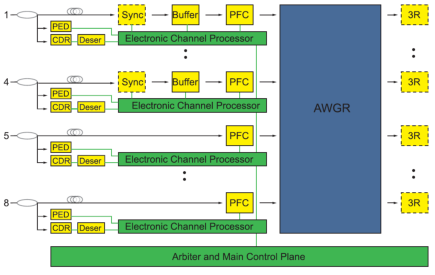
\includegraphics[width=.7\linewidth]{lasor.pdf}
  \caption{Η αρχιτεκτονική του LASOR}
  \label{fig:lasor}
\end{figure}

\subsection{Διερεύνηση και πραγματοποίηση Optical Switch από την ομάδα του U.C.
Santa Barbara στο πλαίσιο της αρχιτεκτονικής LASOR}

Πραγματοποιήθηκε monolithic integration ενός γρήγορου switch fabric
για έναν οπτικό δρομολογητή ενσωματώνοντας 8 MZI-SOA tunable
wavelength converters που λειτουργούν στα 40 Gbps και ενός arrayed
waveguide grating σε ένα μόνο ολοκληρωμένο κύκλωμα. \cite{5515982} Το
ολοκληρωμένο κύκλωμα MOTOR (Monolithic Tunable Optical Router)
περιείχε περισσότερα από 200 ενσωματωμένα λειτουργικά στοιχεία. Η
πλατφόρμα ενσωμάτωσης υποστηρίζει τόσο τα ενεργά, όσο και τα χαμηλής
απώλειας στοιχεία χρησιμοποιώντας μια καινοτόμο, single-regrowht,
quantum-well intermixing προσέγγιση. Αυτή η πλατφόρμα επιτρέπει τη
μείωση των απωλειών απορρόφησης στις περιοχές του AWGR και των delay
lines, εκμεταλλευόμενη ένα undoped InP setback layer στα παθητικά
τμήματα της συσκευής ενώ βελτιστοποιούνται οι ενεργές λειτουργίες.  Το
chip έχει τρεις διαφορετικούς τύπους κυματοδηγοών: έναν κυματοδηγό
surface ridge design στο τμήμα μετατροπής μήκους κύματος, έναν υψηλής
αντίθεσης βαθιά χαραγμένο κυματοδηγό στη delay line για σταθερότητα,
και έναν buried rib κυματοδηγό στην περιοχή του AWGR για τις απώλειες
χαμηλής σκέδασης.

%%% Local Variables:
%%% mode: latex
%%% TeX-master: "main"
%%% TeX-engine: xetex
%%% End:
